\documentclass[main]{subfiles}


\begin{document}
\newpage
\section{Learning In Recurrent Neuronal Networks}
\subsection{Motivation: Why is it so important to understand RNN learning?}
\begin{enumerate}
    \item The mammalian cortex is highly recurrent - it will help us to better understand the brain.
    \item The core reason that recurrent nets are more exciting is that they allow us to operate over sequences of vectors: Sequences in the input, the output, or in the most general case both. Thus better understanding RNNs might help us to develop new, powerful RNN algorithms that are able to learn long and complex sequences.
    \item In programming terms be interpreted as running a fixed program with certain inputs and some internal variables. Viewed this way, RNNs essentially describe programs. In fact, it is known that RNNs are Turing-Complete in the sense that they can be used to simulate arbitrary programs (with proper weights).
    \item RNNs perform exceptionally well in language-modeling, the task of predicting the probability of the next word in a sequence.
\end{enumerate}


\subsection{RNNs in machine learning}
\subsubsection{What is a Recurrent Neural Network? (RECAP)}
\begin{figure}[H]
    \centering
    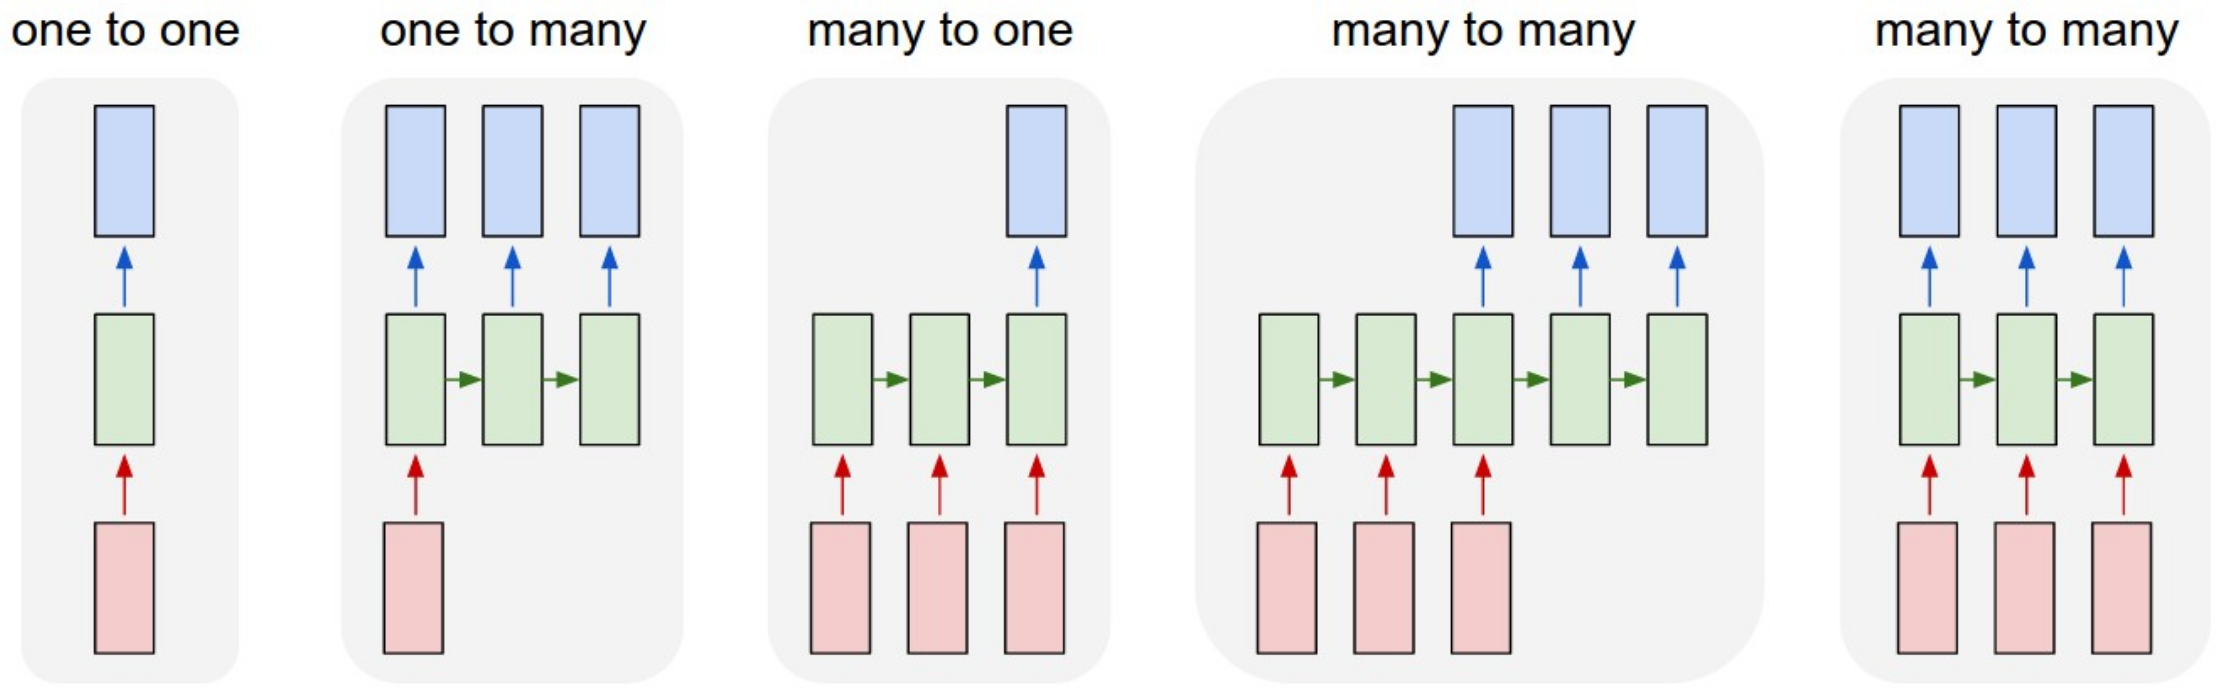
\includegraphics[width=0.99\linewidth]{13_LearningInRecurrentNeuronalNetworks/figures/onetomany.png}
    \caption{Each rectangle is a vector and arrows represent functions (e.g. matrix multiply). Input vectors are in red, output vectors are in blue and green vectors hold the RNN's state (more on this soon). From left to right: \textbf{(1)} Vanilla mode of processing without RNN, from fixed-sized input to fixed-sized output (e.g. image classification). \textbf{(2)} Sequence output (e.g. image captioning takes an image and outputs a sentence of words). \textbf{(3)} Sequence input (e.g. sentiment analysis where a given sentence is classified as expressing positive or negative sentiment). \textbf{(4)} Sequence input and sequence output (e.g. Machine Translation: an RNN reads a sentence in English and then outputs a sentence in French). \textbf{(5)} Synced sequence input and output (e.g. video classification where we wish to label each frame of the video). Notice that in every case are no pre-specified constraints on the lengths sequences because the recurrent transformation (green) is fixed and can be applied as many times as we like.}
    \label{fig:onetomany}
\end{figure}


Recurrent Neural Networks (RNNs) add an interesting twist to basic neural networks. A vanilla neural network takes in a fixed size vector as input which limits its usage in situations that involve a ‘series’ type input with no predetermined size. Recurrent nets allow us to operate over sequences of vectors: Sequences in the input, the output, or in the most general case both (A sequence means, that the elements can have dependency on each other and that the order matters!). A few examples that may make this more concrete\footnote{Cool blog by Karpathy (Teslas AI director): \url{http://karpathy.github.io/2015/05/21/rnn-effectiveness/}}, are shown in \cref{fig:onetomany}. The size of the input or output sequence is flexible, i.e. does not change the architecture of the model. Each network state gets an indices for the sequence. Since the sequence is often related with time progression, the index is choosen to be $t$. The main difference in architecture compared to conventional ANNs is, that recurrent loops are allowed, i.e. inputs from previous layer states of the network. Looking at a one-to-one neural network with one hidden layer, we can write the output state $y(t)$ and the hidden layer state $h(t)$ as follows:

\begin{align*}
    y(t) &= g_y(W_y h(t) + b_y) \tag{1}\\
    h(t) &= g_h(W_x x(t) + W_h h(t-1) + b_h) \tag{2}\\
    &= g_h((W_{hh}W_{xh}) \myvec{h_{t-1}\\ x_t})\\ 
    &= g_h(W \myvec{h_{t-1}\\ x_t}),
\end{align*}
where we include the bias in the W matrix. If we want to display the network over all sequences graphically, i.e. the computational graph, we can unroll it as displayed in \cref{fig:unroll}. 

\begin{figure}[H]
    \centering
    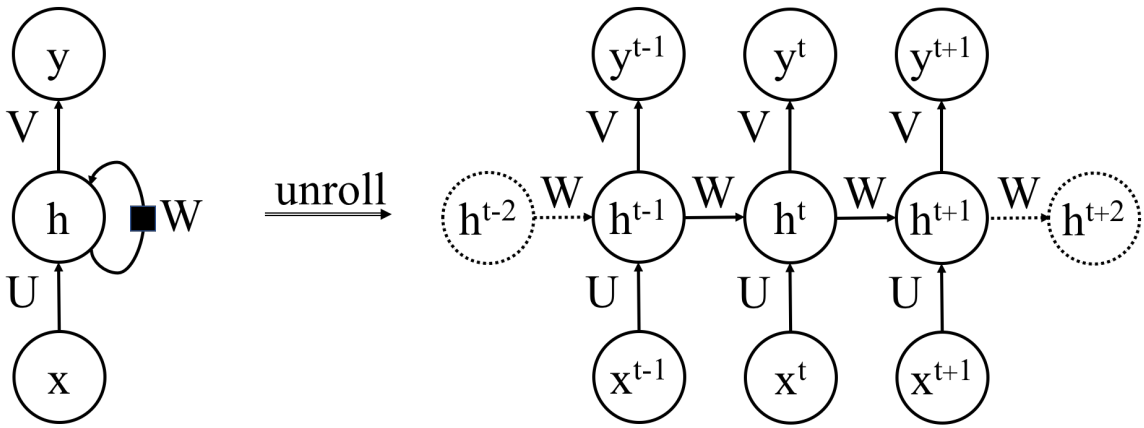
\includegraphics[width=0.99\linewidth]{13_LearningInRecurrentNeuronalNetworks/figures/unrolling.png}
    \caption{Computational graph of a many-to-many network: Unrolling the network over all sequences.}
    \label{fig:unroll}
\end{figure}

This gives us another perspective: For any fixed sequence length $s$, the unrolled recurrent network corresponds to a feedforward network with $s$ hidden layers. The two main differences to a feedforward network is, that the inputs are processed and outputs produced in sequence, and that the same parameters are used for all layers / all time steps, i.e. the same functions $U$, $V$, $W$ applied over all time steps\footnote{Here another helpful entry: \url{https://towardsdatascience.com/recurrent-neural-networks-d4642c9bc7ce}}(Not to be confused with all epochs!!!).

\subsubsection{Back-Propagation Through Time (BPTT)}
The unfolding shown in \cref{fig:unroll} is the first step of a particular network training algorithm, which is called Back-Propagation Through Time (BPTT). The second step is applying our known backpropagation algortihm to the unrolled network to calculate all weight updates. 
%
\begin{figure}[H]
    \centering
    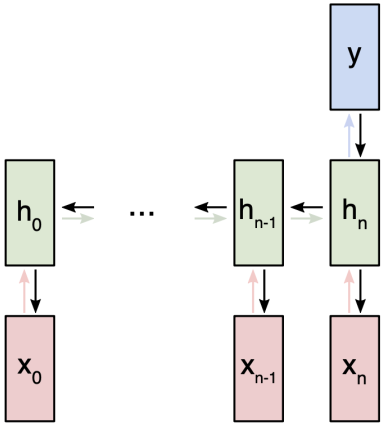
\includegraphics[width=0.5\linewidth]{13_LearningInRecurrentNeuronalNetworks/figures/bptt.png}
    \caption{Illustrating the backpropagation-through-time algorithm on a many-to-one RNN.}
    \label{fig:unroll}
\end{figure}
%
There are several drawbacks to BPTT:
\paragraph{Costly parameter update:} Especially for long sequences, the parameter update for a shallow layer is the same as updating a parameter in an extremely deep feedforward network. One way to fix this is using a truncated BPTT algortithm.  It processes the sequence one timestep at a time, and every $k1$ timesteps, it runs BPTT for $k2$ timesteps, so a parameter update can be cheap if $k2$ is small. Consequently, its hidden states have been exposed to many timesteps and so may contain useful information about the far past, which would be opportunistically exploited\footnote{Sutskever, "Training Recurrent Neural Networks", 2013}.

\paragraph{Exploding gradients:} The gradients coming from the deeper layers have to go through continuous matrix multiplications because of the the chain rule, and as they approach the earlier layers. If they have large values ($>1$) they get larger and eventually blow up and crash the model (NaN-values!). This can be solved by gradient clipping; which places a predefined threshold on the gradients to prevent it from getting too large. Note that this only changes the length, and not the direction, of the gradients.

\paragraph{Vanishing gradients:} A similar problem arises if the gradients have small values ($<1$). They will shrink exponentially until they vanish and make it impossible for the model to learn. This issue cannot be solved as simple; hence it requires to use shorter sequences or to make fundamental change in the RNN architecture. 


\subsubsection{Long-Short-Term-Memory (LSTM) Networks}
Long Short-Term Memory (LSTM) is a feature of a RNN that tackles the problems arising from long sequences / deep networks\footnote{Hochreiter\&Schmidhuber, "Long Short-Term Memory", 1997} \footnote{Great blog post explaining LSTM: \url{http://colah.github.io/posts/2015-08-Understanding-LSTMs/}}. A common LSTM unit is composed of a cell, an input gate \textbf{i}, an output gate \textbf{o}, a forget gate \textbf{f} and a gate gate \textbf{g}. The cell remembers values over arbitrary time intervals and the three gates regulate the flow of information into and out of the cell. A comparison between a normal RNN cell and a LSTM cell is given in the figure below.  
\begin{figure}[H]
    \centering
    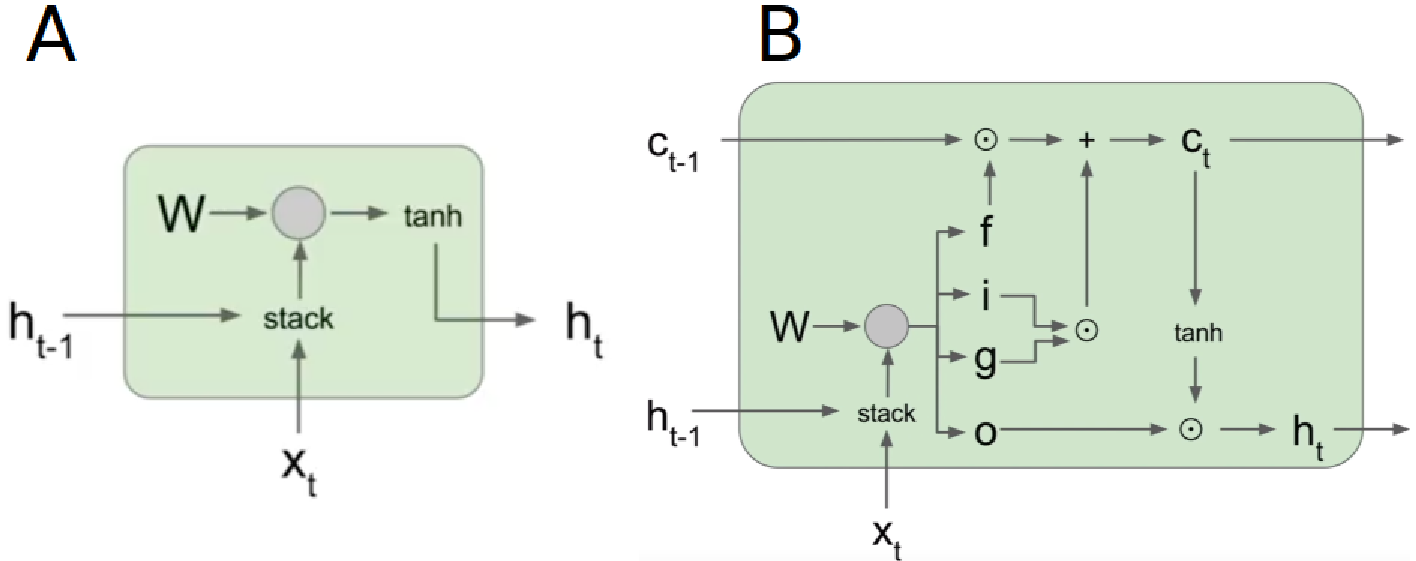
\includegraphics[width=0.99\linewidth]{13_LearningInRecurrentNeuronalNetworks/figures/lstm.png}
    \caption{A comparison between a normal RNN cell \textbf{A} and a LSTM cell \textbf{B}.}
    \label{fig:unroll}
\end{figure}
The gate vector can be written as 
\begin{equation}
    \myvec{i\\ f\\ o\\ g} = \myvec{\sigma\\ \sigma\\ \sigma\\ \tanh} W \myvec{h_{t-1}\\ x_t},
\end{equation}
where $W = \myvec{W_i& W_f& W_o& W_g}.$ The cell state is defined as the following:
\begin{align*}
    c_t = & f \odot c_{t-1} + i \odot g \\
    = &\sigma ( W_{hf} h_{t-1} + W_{xf} x_t ) \odot c_{t-1}\\ 
    + &\sigma ( W_{hi} h_{t-1} + W_{xi} x_t ) \odot \tanh (W_{hg} h_{t-1} + W_{xg} x_t)
\end{align*}
The hidden state is then given by 
\begin{align*}
    h_t &= o \odot \tanh(c_t)\\
    &= \sigma (W_{hho} h_{t-1} + W_{xho} x_t ) \odot \tanh(c_t)
\end{align*}
The practicality of having this particular cell structure is evident if we look at multiple cells at once, i.e. the processing over multiple sequences, as it is done in \cref{fig:lstm_many}. Training works again with Back-propagation-Through-Time. The gradient can now be passed without being interupted, i.e. the problems of costly weight updates, vanishing and exploding gradients should not occur anymore. 
\begin{figure}[H]
    \centering
    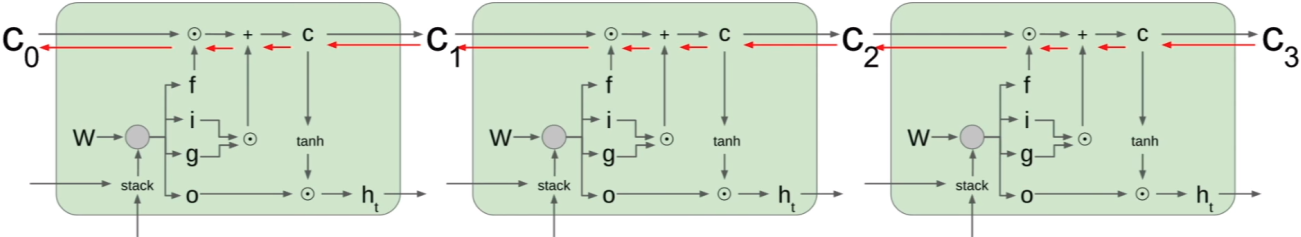
\includegraphics[width=0.99\linewidth]{13_LearningInRecurrentNeuronalNetworks/figures/lstm_many.png}
    \caption{Illustration of LSTM over many sequences. Red arrow denotes the gradient, which can flow uninterruptedly.}
    \label{fig:lstm_many}
\end{figure}





\subsection{RNNs in the Brain}
\subsubsection{Looking at the Cat}
\subsubsection{Looking at the Mouse}
\subsubsection{Looking at the Primate}


\subsection{RNNs in Theoretical Neuroscience}
\subsubsection{Reservoir Computing}
\subsubsection{Learning via Backpropagation Through Time (BPTT)}
\subsubsection{Learning via Real Time Recurrent Learning (RTRL)}
\subsubsection{First-Order, Reduced and Controlled Error (FORCE) Learning}
\subsubsection{Self Organizing Recurrent Networks (SORN)}
\end{document}